
%(BEGIN_QUESTION)
% Copyright 2011, Tony R. Kuphaldt, released under the Creative Commons Attribution License (v 1.0)
% This means you may do almost anything with this work of mine, so long as you give me proper credit

This compressor control system uses a pressure transmitter and controller to regulate the discharge pressure to a constant setpoint, allowing either a power controller (JIC) or a suction pressure controller (PIC) to override.  The power controller overrides the discharge pressure controller under conditions of high load, throttling back the suction valve to limit power.  The suction pressure controller overrides them all under conditions of high inlet vacuum, opening the suction valve in order to ensure the compressor's gland seals are not ruined by excessive vacuum:

$$\includegraphics[width=15.5cm]{i00179x01.eps}$$

In the event of a high inlet vacuum condition simultaneous with a high load condition, the suction pressure controller will ``win'' by overriding the power controller.  Alter this system so that the override priority is vice-versa: the power controller is able to override the suction pressure controller, yet the suction controller is still able to override the discharge controller.

\underbar{file i00179}
%(END_QUESTION)





%(BEGIN_ANSWER)

$$\includegraphics[width=15.5cm]{i00179x02.eps}$$

%(END_ANSWER)





%(BEGIN_NOTES)

%INDEX% Control, strategies: override control
%INDEX% Process: compressor load control
%INDEX% Relay, computational: symbol identification

%(END_NOTES)


